\section{Results} \label{sect:case-study:results}

The result section focuses in showcasing the evaluation of the \mlblink algorithm and comparing it to randomly searching for anomalies in the $\beta$--pack dataset. To do so, the \mlblink algorithm is executed in isolation (i.e. without using the \mlblinkui). The reasoning behind this decision is that it is simpler and faster to evaluate the algorithm without having to depend on whether a user made a good matching or not. In order to enable this, the $\beta$--pack was slightly modified to contain a total of 7 anomalies. These anomalies were created by randomly selecting a few missions, and manually altering them as explained in section \ref{subsect:case-study:intro:matching-accuracy} and shown in figure \ref{fig:fake:mission-13}. All anomalies consisted of removing objects close to the center from \panstarrs that are discernible in their \usno equivalent. Through out this section, the notation ``\texttt{image\_key}.\texttt{usno\_band}.\texttt{panstarr\_band}'' will be used to refer to an image of the $\beta$--pack dataset. \newline

As seen in table \ref{table:case-study:intro:datasets-mapping}, some \panstarrs color--bands are mapped into multiple \usno color--bands. For instance, if a \panstarrs anomaly is manually created in color--band \texttt{g}, it must be mapped to both \usno \texttt{blue1} and \texttt{blue2}. Therefore, that single anomaly actually counts as two, since the \mlblink algorithm is expected to find it across the two \usno bands. Table \ref{table:results:anomalies-list} shows the complete list of fake anomalies that were created to evaluate the algorithm. \newline

\begin{table}[H]
    \centering
        \begin{tabular}{| c | c | c |}
            \hline
              Image Key & \usno Band & \panstarrs Band \\
            \hline
              13 & \texttt{blue1} & \texttt{g} \\
            \hline
              13 & \texttt{blue2} & \texttt{g} \\
            \hline
              56 & \texttt{blue1} & \texttt{g} \\
            \hline
              56 & \texttt{blue2} & \texttt{g} \\
            \hline
              679 & \texttt{ir} & \texttt{z} \\
            \hline
              831 & \texttt{red1} & \texttt{r} \\
            \hline
              831 & \texttt{red2} & \texttt{r} \\
            \hline
        \end{tabular}
    \caption{Complete list of anomalies that were created to evaluate the \mlblink algorithm.}
    \label{table:results:anomalies-list}
\end{table}

A naive solution for the requirements of the \vasco project would simply randomly attempt to find the anomalies in the $\beta$--pack. Since there are a total of $5005$ observations in the $\beta$--pack, a random recommender system would recommend an item with probability of $1/5005 = 0.0002$. Furthermore, the \mlblink algorithm will be tested by executing it for $200$ time steps. A random recommender system that is ran $200$ times, with the goal of finding $7$ anomalies in a dataset of $5005$ observations would be expected to find $7 \times 1/5005 \times 200 = 0.27$ anomalies. \newline

Figure \ref{fig:evaluation:roc-curve} shows the ROC curve created by running the \mlblink algorithm for 200 time steps. The image vectors were reduced to 250 projections, and the binarization thresholds for \usno and \panstarrs were 60 and 220 respectively. These parameters were adjusted using trial and error by analyzing the results of the ROC curve, AUC, and the number of anomalies found during the specified number of time steps in the experiments. While there is some randomization involved in the algorithm, with the parameters previously specified the results are easily reproducible: the \mlblink algorithm consistently achieves an AUC around $0.70$, and finds 2 up to 4 anomalies out of 7. In the experiment shown in figure \ref{fig:evaluation:roc-curve}, the \mlblink algorithm found 3/7 anomalies, and achieved the best $\text{AUC} = 0.77$ at $t = 100$. \newline

\begin{figure}
  \centering
  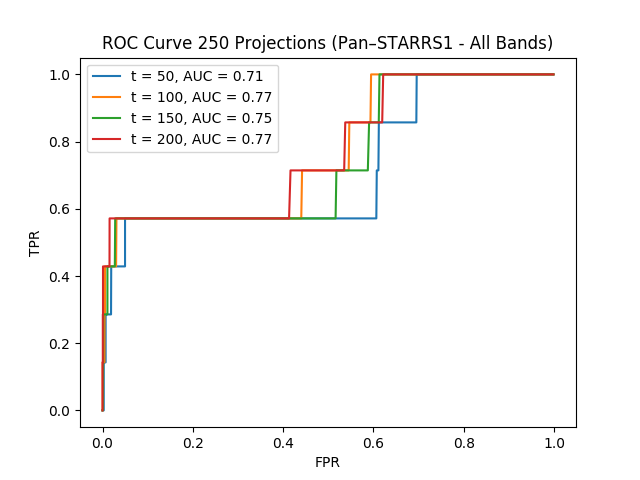
\includegraphics[
        width=0.7\textwidth,
        keepaspectratio
  ]{report/images/results/250_all_bands/250_all_bands_3_anomalies_t_200.png}
  \caption{ROC curve and AUC of the evaluation of the \mlblink algorithm using 250 projections for a total of 200 time steps.}
  \label{fig:evaluation:roc-curve}
\end{figure}

As explained in section \ref{sect:meth:evaluation}, the discrimination threshold used to create the ROC curve is ``sweeping'' the entire range of $v$ values from $\min(v)$ up to $\max(v)$ in a time step $t$. It is thus reasonable that for all time steps, the ROC curve in figure \ref{fig:evaluation:roc-curve} starts with an ascend (i.e. more true positives) since the $v$ value is small and we expect more anomalies to evaluate to a $v$ value in that range. On the other hand, as the discrimination threshold is increased, the false positives rate starts to catch up and eventually dominates the ROC curve. The \mlblink algorithm was consistently able to find the first 2 or 4 anomalies listed in table \ref{table:results:anomalies-list}, but it could not find the last 3 - even when more time steps were used in the evaluation. This is also why the ROC curve in figure \ref{fig:evaluation:roc-curve} has three ``steps'' before reaching a $\text{TPR} = 1.0$; these three steps are the 3 anomalies that the \mlblink algorithm is unable to find because their $v$ value is too large. \newline

Figure \ref{fig:evaluation:v-versus-t:found} shows how the $v$ value of known anomalies that were found versus a normal observation changes as the \mlblink algorithm is taught over time. Additionally, the figure includes the $\min(v)$ value at each time step. As expected, the $v$ value of the known anomalies is close to the $\min(v)$ value of each time step, while the normal observation results in a larger $v$ value. Note the $v$ value of an anomaly might be smaller than the $\min(v)$ of a time step only after it has been found. The reason for this is that once an anomaly is found, it is filtered out of the potential candidates to be crawled, otherwise the \mlblink algorithm will continue to recommend it. In this scenario, the $v$ value of an anomaly was computed after it has been found for illustrative purposes only. The anomalies in figure \ref{fig:evaluation:v-versus-t:found} were found in the following order: \texttt{13.blue2.g} in $t = 110$, \texttt{56.blue2.g} at $t = 158$, and finally \texttt{56.blue1.g} in $t = 189$. \newline

\begin{figure}
  \centering
  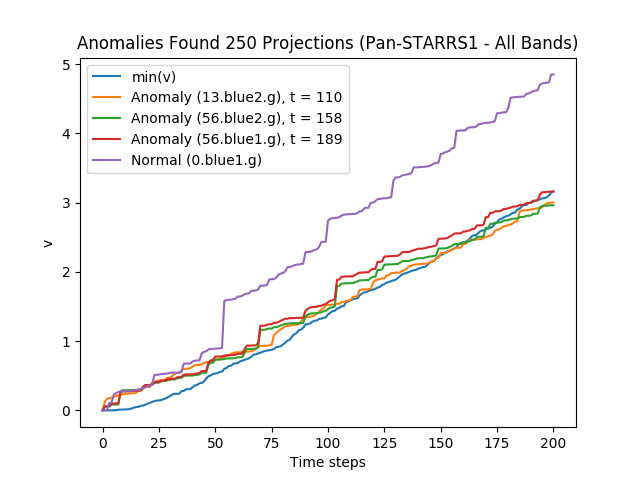
\includegraphics[
        width=0.7\textwidth,
        keepaspectratio
  ]{report/images/results/250_all_bands/found_250_all_bands_3_anomalies_t_200.png}
  \caption{Evaluation of known anomalies (that the \mlblink algorithm found) versus normal observations in comparison to the $\min(v)$ value at each time step.}
  \label{fig:evaluation:v-versus-t:found}
\end{figure}

The same plot is shown in figure \ref{fig:evaluation:v-versus-t:not-found}, but this time it shows the anomalies the \mlblink algorithm could not find. Except for anomaly \texttt{13.blue1.g}, the results are the opposite of what is expected, since the $v$ value of the anomalies is closer to the normal observation than it is to the $\min(v)$ value at each time step. \newline

\begin{figure}
  \centering
  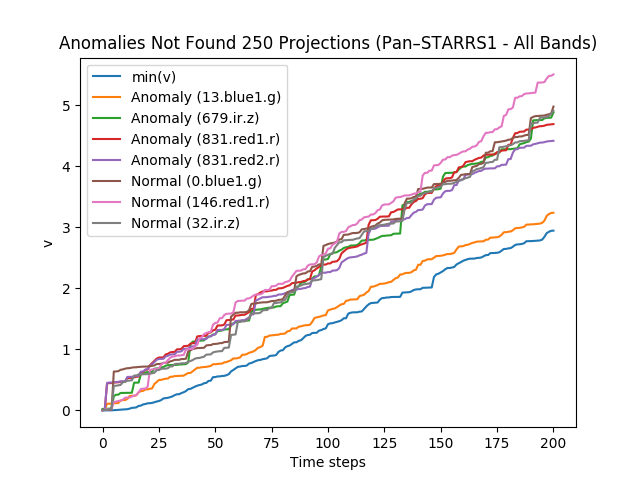
\includegraphics[
        width=0.7\textwidth,
        keepaspectratio
  ]{report/images/results/250_all_bands/not_found_250_all_bands_4_anomalies_t_200.png}
  \caption{Evaluation of known anomalies (that the \mlblink algorithm could not find) versus normal observations in comparison to the $\min(v)$ value at each time step.}
  \label{fig:evaluation:v-versus-t:not-found}
\end{figure}

The common denominator of the 4 anomalies the \mlblink algorithm evaluated to be close to the $\min(v)$ value of any time step is that these are all defined in the \texttt{g} color--band of \panstarrs. To further understand the capabilities of the \mlblink algorithm when using projections for dimensionality reduction, each \panstarrs band was evaluated in isolation. The experiments were conducted one \panstarrs band at a time. That is, \panstarrs color--band \texttt{g} (versus \usno color--bands \texttt{blue1} and \texttt{blue2}) with a total of $2002$ observations and $4$ fake anomalies was tested in isolation. Next, \panstarrs color--band \texttt{r} (versus \usno color--bands \texttt{red1} and \texttt{red2}) with a total of $2002$ observations and $2$ fake anomalies was evaluated next. Finally, \panstarrs color--band \texttt{z} (versus \usno color--band \texttt{ir}) with a total of $1001$ observations and $1$ fake anomaly was tested. \newline

%%%%%%%%%%%% PanSTARR band g %%%%%%%%%%%%

Figure \ref{fig:evaluation:roc:panstarrs:g} shows the ROC and AUC achieved by \mlblink when evaluating the \panstarrs color--band \texttt{g} in isolation. As expected, \mlblink does very well, consistently achieving an AUC of at least $0.90$ for all time steps shown in the plot. It found $3$ out of $4$ anomalies in the following order: \texttt{56.blue2.g} in $t = 62$, \texttt{13.blue2.g} at $t = 82$, and \texttt{56.blue1.g} in $t = 105$. Figure \ref{fig:evaluation:found:panstarrs:g} shows the evaluation of the $v$ value of known anomalies (that were found when testing \panstarrs color--band \texttt{g} in isolation) versus a normal observation. Once again, as expected, the plot shows \mlblink consistently evaluates the $v$ value of known anomalies to be significantly smaller than that of a normal observation.

\begin{figure}[H]
  \centering
  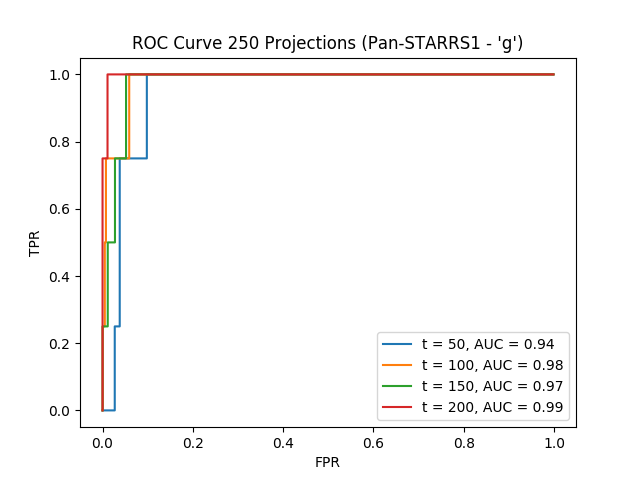
\includegraphics[
        width=0.7\textwidth,
        keepaspectratio
  ]{report/images/results/250_panstarr_g/250_panstarr_g_3_anomalies_t_200.png}
  \caption{ROC curve and AUC achieved by the \mlblink algorithm when evaluating observations in the \panstarrs color--band \texttt{g} only (versus \usno color--bands \texttt{blue1} and \texttt{blue2}) using 250 projections for dimensionality reduction.}
  \label{fig:evaluation:roc:panstarrs:g}
\end{figure}

\begin{figure}[H]
  \centering
  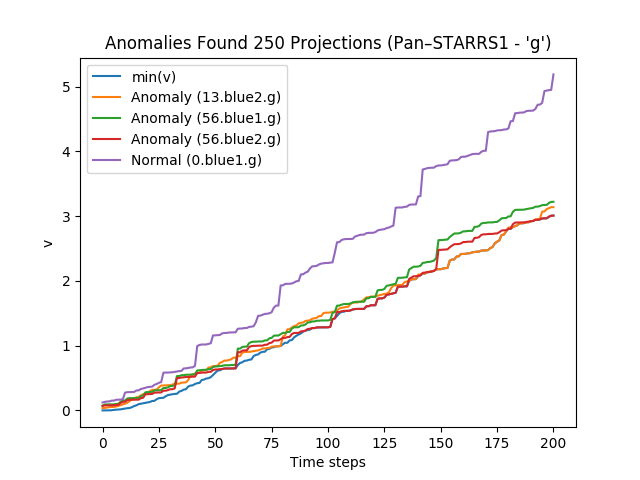
\includegraphics[
        width=0.7\textwidth,
        keepaspectratio
  ]{report/images/results/250_panstarr_g/found_250_panstarr_g_3_anomalies_t_200.png}
  \caption{Evaluation of known anomalies that were found by the \mlblink algorithm when evaluating the \panstarrs color--band \texttt{g} (versus \usno color--bands \texttt{blue1} and \texttt{blue2}) in isolation using 250 projections for dimensionality reduction.}
  \label{fig:evaluation:found:panstarrs:g}
\end{figure}

%%%%%%%%%%%% PanSTARR band r %%%%%%%%%%%%

Figure \ref{fig:evaluation:roc:panstarrs:r} shows the ROC and AUC of the evaluation of the \panstarrs \texttt{r} band in isolation. The results achieved are quite poor: it does not find any anomalies (out of $2$), and achieves an AUC in the $0.5$ range. Figure \ref{fig:evaluation:not-found:panstarrs:r} shows the \mlblink algorithm evaluates the anomalies in the dataset as if these were normal observations (their $v$ values are closer to that of a normal observation than to the $\min(v)$ of any time step).

\begin{figure}[H]
  \centering
  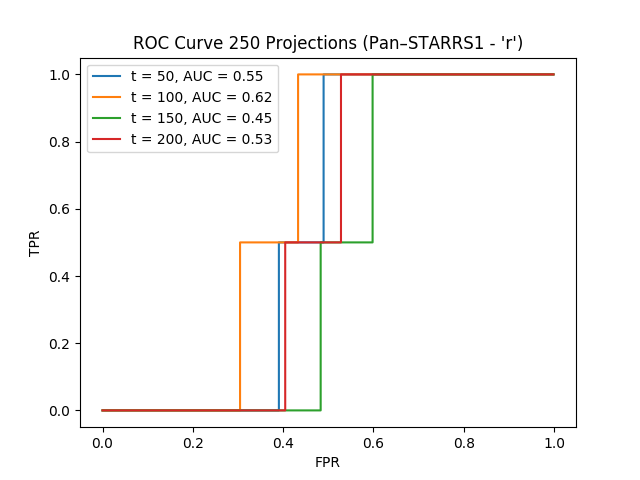
\includegraphics[
        width=0.7\textwidth,
        keepaspectratio
  ]{report/images/results/250_panstarr_r/250_panstarr_r_0_anomalies_t_200.png}
  \caption{ROC curve and AUC achieved by the \mlblink algorithm when evaluating observations in the \panstarrs color--band \texttt{r} only (versus \usno color--bands \texttt{red1} and \texttt{red2}) using 250 projections for dimensionality reduction.}
  \label{fig:evaluation:roc:panstarrs:r}
\end{figure}

\begin{figure}[H]
  \centering
  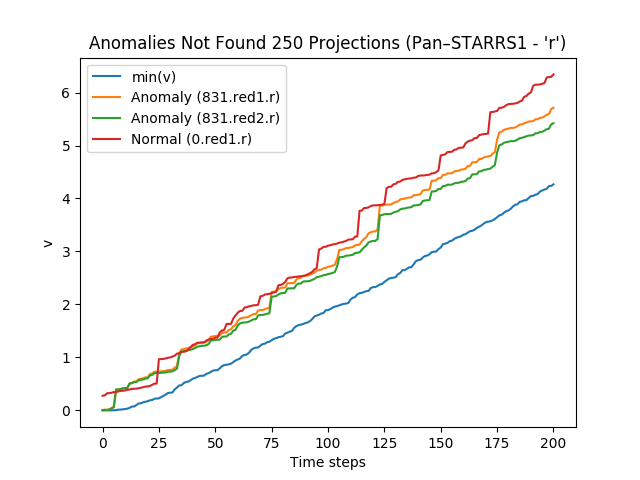
\includegraphics[
        width=0.7\textwidth,
        keepaspectratio
  ]{report/images/results/250_panstarr_r/not_found_250_panstarr_r_2_anomalies_t_200.png}
  \caption{Evaluation of known anomalies that were not found by the \mlblink algorithm when evaluating the \panstarrs color--band \texttt{r} (versus \usno color--bands \texttt{red1} and \texttt{red2}) in isolation using 250 projections for dimensionality reduction.}
  \label{fig:evaluation:not-found:panstarrs:r}
\end{figure}

%%%%%%%%%%%% PanSTARR band z %%%%%%%%%%%%

The results of the evaluation of \panstarrs color--band \texttt{z} are shown in figures \ref{fig:evaluation:roc:panstarrs:z} and \ref{fig:evaluation:not-found:panstarrs:z}. Once again, the \mlblink algorithm performance is poor, with an overall AUC lower than $0.5$, and unable to find the single anomaly defined in this experiment (\texttt{679.ir.z}). Moreover, similar to figure \ref{fig:evaluation:not-found:panstarrs:r}, the \mlblink algorithm consistently evaluates the known anomaly closer to a normal observation than to the $\min(v)$ value of any time step.

\begin{figure}[H]
  \centering
  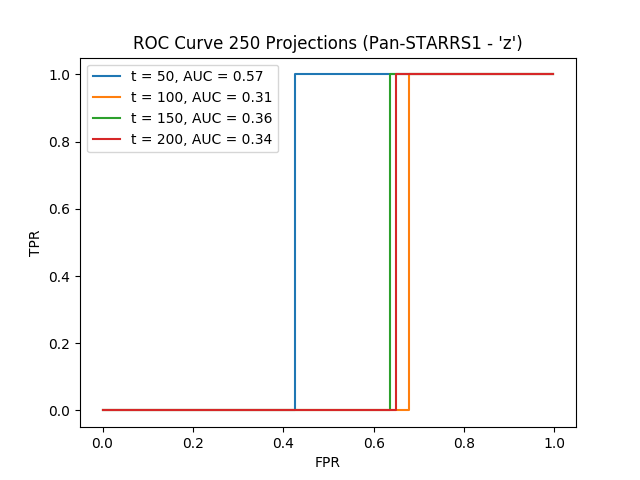
\includegraphics[
        width=0.7\textwidth,
        keepaspectratio
  ]{report/images/results/250_panstarr_z/250_panstarr_z_0_anomalies_t_200.png}
  \caption{ROC curve and AUC achieved by the \mlblink algorithm when evaluating observations in the \panstarrs color--band \texttt{z} only (versus \usno color--band \texttt{ir}) using 250 projections for dimensionality reduction.}
  \label{fig:evaluation:roc:panstarrs:z}
\end{figure}

\begin{figure}[H]
  \centering
  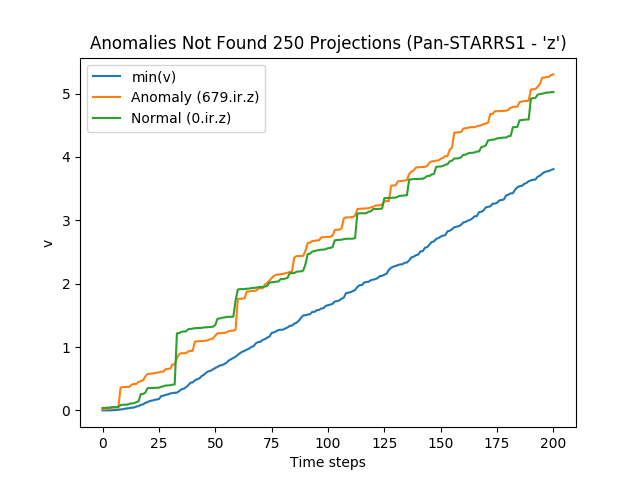
\includegraphics[
        width=0.7\textwidth,
        keepaspectratio
  ]{report/images/results/250_panstarr_z/not_found_250_panstarr_z_1_anomalies_t_200.png}
  \caption{Evaluation of known anomalies that were not found by the \mlblink algorithm when evaluating the \panstarrs color--band \texttt{z} (versus \usno color--bands \texttt{ir}) in isolation using 250 projections for dimensionality reduction.}
  \label{fig:evaluation:not-found:panstarrs:z}
\end{figure}

%%%%%%%%%%%% Average Pooling %%%%%%%%%%%%

The same experiments were conducted but using average pooling with a kernel of size $7 \times 7$ for dimensionality reduction instead. The binarization thresholds for \usno and \panstarrs remained equal as when using projections. \newline

The results of the \mlblink algorithm when using average pooling for dimensionality reduction were unstable and difficult to reproduce. Figure \ref{fig:evaluation:avg-pool:roc} shows the ROC curve for two independent evaluations of the \mlblink algorithm using average pooling for dimensionality reduction for a total of $200$ time steps. \newline

While it was able to find $2$--$3$ anomalies, the AUC in sub--figure \ref{fig:evaluation:avg-pool:roc:a} deviates from $0.54$ at $t = 150$ up to $0.90$ in $t = 50$, and from $0.50$ in $t = 200$ up to $0.82$ at $t = 150$ in sub--figure \ref{fig:evaluation:avg-pool:roc:b}. This suggests the representation of the learned weights in the matrix $\vect{D}$ when using average pooling for dimensionality reduction is volatile, and small changes of the members that are inserted in the active set can greatly affect the outcome of the model.

\begin{figure}[H]
    \centering
    \begin{subfigure}{.5\textwidth}
      \centering
      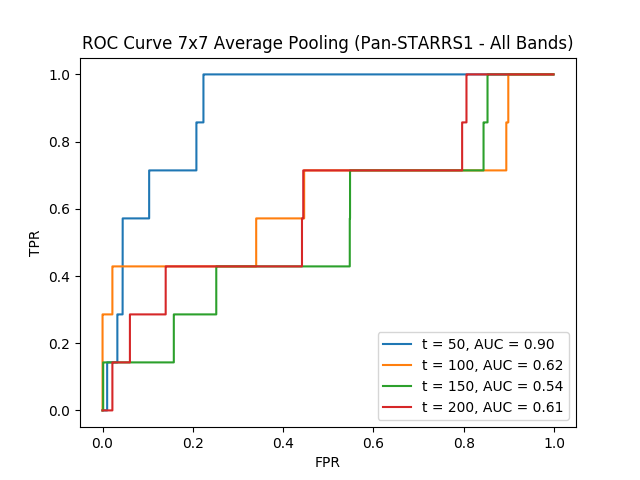
\includegraphics[
            width=\textwidth,
            keepaspectratio
        ]{report/images/results/7x7_all_bands_2/7x7_all_bands_3_anomalies_t_200.png}
      \caption{Experiment 1 ROC Curve and AUC}
      \label{fig:evaluation:avg-pool:roc:a}
    \end{subfigure}%
    \begin{subfigure}{.5\textwidth}
      \centering
      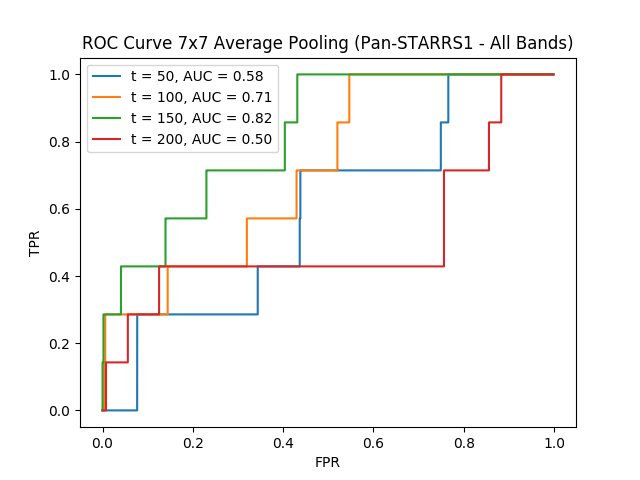
\includegraphics[
            width=\textwidth,
            keepaspectratio
      ]{report/images/results/7x7_all_bands_4/7x7_all_bands_2_anomalies_t_200.png}
      \caption{Experiment 2 ROC Curve and AUC}
      \label{fig:evaluation:avg-pool:roc:b}
    \end{subfigure}
    \caption{ROC curve and AUC of two independent runs of the ML-Blink algorithm when using average pooling with a kernel of size $7 \times 7$ for a total of 200 time steps. The AUC in sub--figure \ref{fig:evaluation:avg-pool:roc:a} deviates from $0.54$ at $t = 150$ up to $0.90$ in $t = 50$, while the AUC of sub--figure \ref{fig:evaluation:avg-pool:roc:b} goes from $0.50$ in $t = 200$ up to $0.82$ at $t = 150$. The large changes in the AUC suggest the representation of the learned weights in the matrix $\vect{D}$ is volatile.}
    \label{fig:evaluation:avg-pool:roc}
\end{figure}

The instability can be better visualized when analyzing the $v$ value of known anomalies versus a normal observation as the \mlblink algorithm is taught over time. Figure \ref{fig:evaluation:avg-pool:v-vs-t} shows a plot of anomalies the \mlblink algorithm found versus a normal observation for $200$ time steps for both experiments in figure \ref{fig:evaluation:avg-pool:roc}. Note the $v$ value of the known anomalies in sub--figure \ref{fig:evaluation:avg-pool:v-vs-t:b} increases towards the end, and it goes even higher than the $v$ value of a normal observation. This behavior is the opposite of what the \mlblink algorithm is designed to do, which suggests average pooling with the configuration used when running these experiments does not capture a good representation of the features that are required to learn what is an anomaly. Additionally, the range of $v$ values the \mlblink computes in sub--figure \ref{fig:evaluation:avg-pool:v-vs-t:a} goes from $0$ up to $0.40$, while in sub--figure \ref{fig:evaluation:avg-pool:v-vs-t:b} it is from $0$ until $0.80$. When using projections, the $v$ values grow is smoother and typically ranges in the $0$--$6$ range regardless of what \panstarrs band is being crawled.

\begin{figure}[H]
    \centering
    \begin{subfigure}{.5\textwidth}
      \centering
      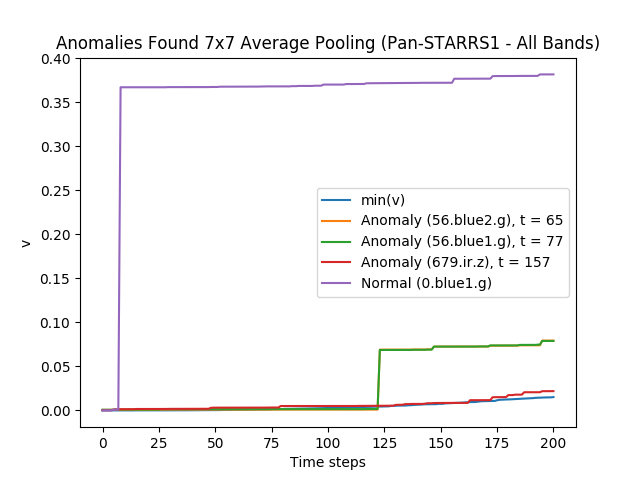
\includegraphics[
            width=\textwidth,
            keepaspectratio
        ]{report/images/results/7x7_all_bands_2/found_7x7_all_bands_3_anomalies_t_200.png}
      \caption{Experiment 1 Anomalies Found}
      \label{fig:evaluation:avg-pool:v-vs-t:a}
    \end{subfigure}%
    \begin{subfigure}{.5\textwidth}
      \centering
      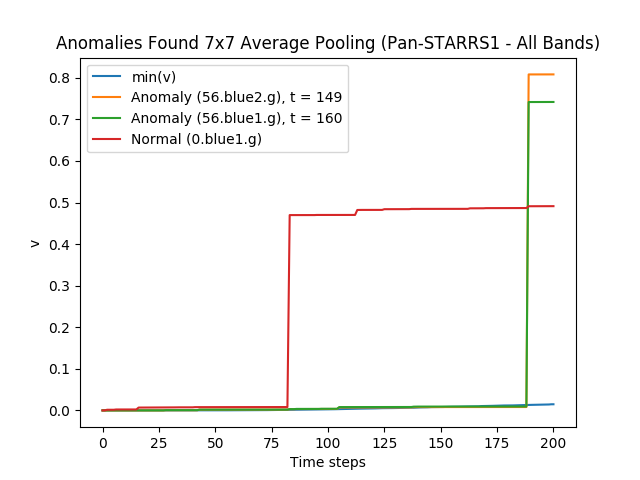
\includegraphics[
            width=\textwidth,
            keepaspectratio
      ]{report/images/results/7x7_all_bands_4/found_7x7_all_bands_2_anomalies_t_200.png}
      \caption{Experiment 2 Anomalies Found}
      \label{fig:evaluation:avg-pool:v-vs-t:b}
    \end{subfigure}
    \caption{Evaluation of the $v$ value of known anomalies and a normal observation as the \mlblink algorithm is taught over time when using average pooling for dimensionality reduction. Notice the unstable change of the $v$ value of the observations in comparison to using projections for dimensionality reduction (figure \ref{fig:evaluation:v-versus-t:found}).}
    \label{fig:evaluation:avg-pool:v-vs-t}
\end{figure}

Similar results were obtained in other experiments when using average pooling for dimensionality reduction (both when crawling all \panstarrs color--bands or one at a time). The only major difference being that sometimes it would find the \texttt{679.ir.z} anomaly (as seen in sub--figure \ref{fig:evaluation:avg-pool:v-vs-t:a}), which projections could not. Regardless of that, the results obtained from multiple runs were highly volatile, and it was decided to not continue these experiments further due to their instability and lack of reproducibility. \newline

Overall, when using all \panstarrs color--bands and projections for dimensionality reduction as seen in figure \ref{fig:evaluation:roc-curve}, the \mlblink algorithm performs substantially better than randomly predicting the label of an observation. It also finds more anomalies when crawling $5005$ observations (all \panstarrs color--bands) than what a random recommender system would be expected to do (i.e. $3 > 0.27$). Nonetheless, these results are primarily determined by the good performance of the \mlblink algorithm in the \panstarrs color--band \texttt{g}. The \mlblink algorithm performance significantly degrades when crawling the \panstarrs color--bands \texttt{r} and \texttt{z}. For both of these color--bands, it was shown the \mlblink algorithm achieves an AUC in the $0.5$ range (or worse). Additionally, when crawling the \panstarrs color--bands \texttt{r} and \texttt{z} in isolation, the \mlblink algorithm was unable to find any of the fake anomalies defined in these color--bands.
